\input{../../../../.preambles/02-lab_work}
\newgeometry{top=1.5cm, bottom=1.5cm, left=1cm, right=1cm}
\begin{document}
    \begin{table}[h!]
        \center
        \begin{tabular}{|C{.5}|C{.2}|C{.25}|}
            \hline
            \multicolumn{1}{|c|}{\multirow{4}{*}{Лабораторная работа № 2}} &
            Студент, группа & {{ student }}, Ф-369 \\ \cline{2-3}
            & Дата выполнения & 16.02.2013 \\ \cline{2-3}
            & Подпись &  \\ \cline{2-3}
            Измерение дозы излучения радиоактивных изотопов & Дата отчёта & \\ \cline{2-3}
            при различных расстояниях от источника & Оценка &  \\ \cline{2-3}
            & Подпись &  \\ \hline
        \end{tabular}
    \end{table}

    \emph{Цель работы:} измерение дозы излучения радиоактивных изотопов при
    различных расстояниях до источника.

    \begin{table}[h!]
        \center
        \begin{tabular}{|c|*{4}{C{.2}|}} \hline
            № & Изотоп & \( T_{1/2} \) & \( n, \% \) & \( A \), Ки \\ \hline
            1 & Радий \( ^{226} \)Ra & 1608 лет & 0,5 & 397,27 \\ \hline
            2 & Ванадий \( ^{48} \)V & 15,97 суток & 0,25 & 7,30 \( \cdot 10^6
            \) \\ \hline
            3 & Цезий \( ^{137} \)Cs & 30 лет & 0,6 & 25,55 \( \cdot 10^3 \) \\
            \hline
            4 & Цинк \( ^{65} \)Zn & 243,5 суток & 0,5 & 955,98 \( \cdot 10^3 \)
            \\ \hline
            5 & Ксенон \( ^{133} \)Xe & 5,25 суток & 0,5 & 44,41 \( \cdot 10^6
            \) \\ \hline
        \end{tabular}
    \end{table}
    
    \subsection{Радий-226 \( \left(^{226}\mathrm{Ra}\right) \)}
    
    \begin{table}[h!]
        \center
        \begin{tabular}{|C{.085}|*{13}{C{.045}|}} \hline
            \( l \), м & 20 & 21 & 22 & 23 & 24 & 25 & 26 & 27 & 28 & 29 & 30
            & 31 & 32 \\ \hline
            % -------------------------------------------------------
            \multirow{3}{*}{\( P \), мкЗв/ч} & 30,69 & 27,72 & 24,11 & 23,95
            & 23,35 & 19,53 & 17,77 & 16,25 & 15,00 & 14,34 & 13,85 & 13,85
            & 11,92 \\ \cline{2-14}
            & 34,20 & 29,57 & 24,80 & 22,92 & 21,72 & 21,62 & 18,52 & 16,01
            & 15,75 & 13,86 & 12,94 & 12,74 & 12,00 \\ \cline{2-14}
            & 33,07 & 26,66 & 26,02 & 23,33 & 20,20 & 20,18 & 18,28 & 16,44
            & 15,71 & 14,05 & 13,95 & 13,54 & 12,91 \\ \hline
            Среднее & 32,65 & 27,98 & 24,98 & 23,40 & 21,77 & 20,44 & 18,19
            & 16,23 & 15,49 & 14,08 & 13,58 & 13,38 & 12,30 \\ \hline
            \multirow{3}{*}{\( P \), мР/ч} & 3,12 & 2,89 & 2,75 & 2,31 & 2,15
            & 1,98 & 1,82 & 1,66 & 1,54 & 1,48 & 1,36 & 1,32 & 1,25 \\ \cline{2-14}
            & 3,43 & 2,80 & 2,78 & 2,34 & 2,25 & 1,93 & 1,87 & 1,79 & 1,68
            & 1,67 & 1,50 & 1,44 & 1,29 \\ \cline{2-14}
            & 3,18 & 3,07 & 2,62 & 2,60 & 2,47 & 2,09 & 1,99 & 1,75 & 1,54
            & 1,53 & 1,46 & 1,26 & 1,24 \\ \hline
            Среднее & 3,24 & 2,95 & 2,72 & 2,42 & 2,29 & 2,00 & 1,89 & 1,73
            & 1,59 & 1,56 & 1,44 & 1,34 & 1,26 \\ \hline
        \end{tabular}
    \end{table}
    
    \begin{figure}[h!]
        \center
        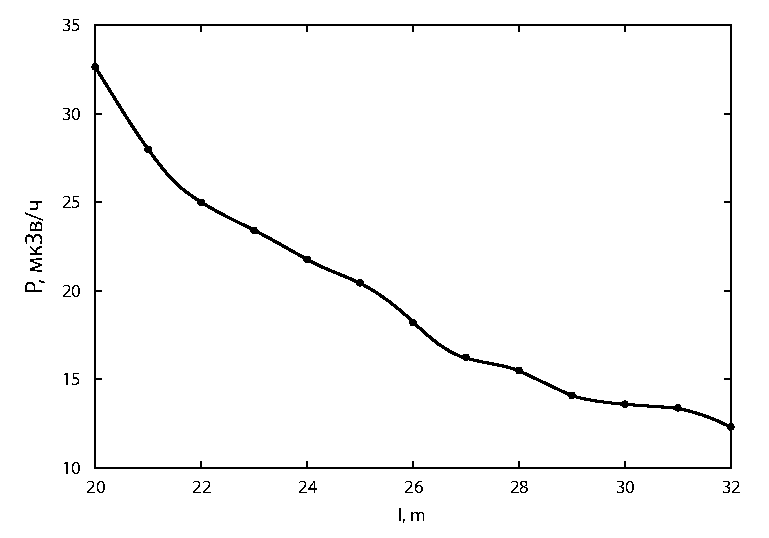
\includegraphics[width=.6\textwidth]{Ra}
        \parbox{.6\textwidth}{\caption{График зависимости \( \midnum{P}(l) \)
        для Радия-226}}
    \end{figure}

    \pagebreak % ---------------------------------------------------------------
    
    \subsection{Ванадий-48 \( \left(^{48}\mathrm{V}\right) \)}
    
    \begin{table}[h!]
        \center
        \begin{tabular}{|C{.065}|*{13}{C{.047}|}} \hline
            \( l \), м & 20 & 21 & 22 & 23 & 24 & 25 & 26 & 27 & 28 & 29 & 30
            & 31 & 32 \\ \hline
            % -------------------------------------------------------
            \multirow{3}{*}{\( P \), Зв/ч} & 249,86 & 236,41 & 211,84 & 197,32
            & 173,26 & 162,33 & 160,52 & 148,36 & 140,36 & 129,59 & 123,31
            & 115,83 & 99,69 \\ \cline{2-14}
            & 258,54 & 258,46 & 230,27 & 222,75 & 177,42 & 175,28 & 156,91
            & 150,77 & 147,96 & 124,53 & 121,61 & 113,22 & 100,28
            \\ \cline{2-14}
            & 278,36 & 237,91 & 220,33 & 187,78 & 172,72 & 168,04 & 162,26
            & 150,65 & 149,12 & 125,01 & 111,08 & 111,03 & 106,03 \\ \hline
            Среднее & 262,25 & 244,26 & 220,21 & 202,62 & 174,47 & 168,55
            & 160,00 & 149,93 & 145,81 & 126,38 & 118,67 & 113,36 & 102,00 \\ \hline
            \multirow{3}{*}{\( P \), кР/ч} & 26,14 & 24,39 & 23,41 & 21,28
            & 20,23 & 19,20 & 15,07 & 14,26 & 13,72 & 12,73 & 12,62 & 11,56
            & 10,73 \\ \cline{2-14}
            & 30,85 & 24,09 & 21,14 & 20,76 & 18,73 & 18,56 & 16,26 & 14,67
            & 13,84 & 13,30 & 12,81 & 12,59 & 10,43 \\ \cline{2-14}
            & 29,70 & 24,34 & 23,10 & 21,56 & 18,46 & 17,00 & 15,80 & 14,41
            & 13,38 & 12,19 & 12,08 & 11,54 & 10,25 \\ \hline
            Среднее & 28,90 & 24,27 & 22,55 & 21,20 & 19,14 & 18,25 & 15,71
            & 14,45 & 13,65 & 12,74 & 12,50 & 11,90 & 10,47 \\ \hline
        \end{tabular}
    \end{table}
    
    \subsection{Цезий-137 \( \left(^{137}\mathrm{Cs}\right) \)} % ---------------
    
    \begin{table}[h!]
        \center
        \begin{tabular}{|C{.07}|*{13}{C{.047}|}} \hline
            \( l \), м & 20 & 21 & 22 & 23 & 24 & 25 & 26 & 27 & 28 & 29 & 30
            & 31 & 32 \\ \hline
            % -------------------------------------------------------
            \multirow{3}{*}{\( P \), мЗв/ч} & 207,56 & 188,84 & 181,63 & 167,64
            & 150,32 & 121,28 & 112,82 & 104,19 & 98,66 & 93,06 & 83,77 & 79,87
            & 73,65 \\ \cline{2-14}
            & 187,94 & 170,13 & 168,06 & 157,64 & 130,85 & 119,21 & 113,47
            & 103,69 & 101,57 & 95,71 & 84,86 & 80,89 & 70,99 \\ \cline{2-14}
            & 210,02 & 170,42 & 163,03 & 139,88 & 133,43 & 123,81 & 112,13
            & 106,94 & 102,83 & 102,60 & 84,61 & 79,03 & 72,89 \\ \hline
            Среднее & 201,84 & 176,46 & 170,91 & 155,05 & 138,20 & 121,43
            & 112,81 & 104,94 & 98,99 & 97,12 & 84,41 & 79,93 & 72,51 \\ \hline
            \multirow{3}{*}{\( P \), Р/ч} & 21,76 & 17,46 & 16,92 & 16,41
            & 14,97 & 13,65 & 11,41 & 11,28 & 10,14 & 9,83 & 9,71 & 8,26 & 7,94
            \\ \cline{2-14}
            & 21,35 & 19,83 & 16,91 & 14,91 & 14,61 & 14,12 & 12,71 & 10,28
            & 10,20 & 10,06 & 8,68 & 8,42 & 8,04 \\ \cline{2-14}
            & 22,09 & 17,90 & 16,37 & 14,73 & 13,83 & 13,79 & 12,13 & 10,83
            & 10,29 & 9,61 & 8,32 & 8,32 & 8,16 \\ \hline
            Среднее & 21,73 & 18,25 & 16,37 & 15,35 & 14,47 & 13,85 & 12,08
            & 10,80 & 10,21 & 9,83 & 8,91 & 8,33 & 8,05 \\ \hline
        \end{tabular}
    \end{table}
    
    \begin{figure}[h!]
        \center
        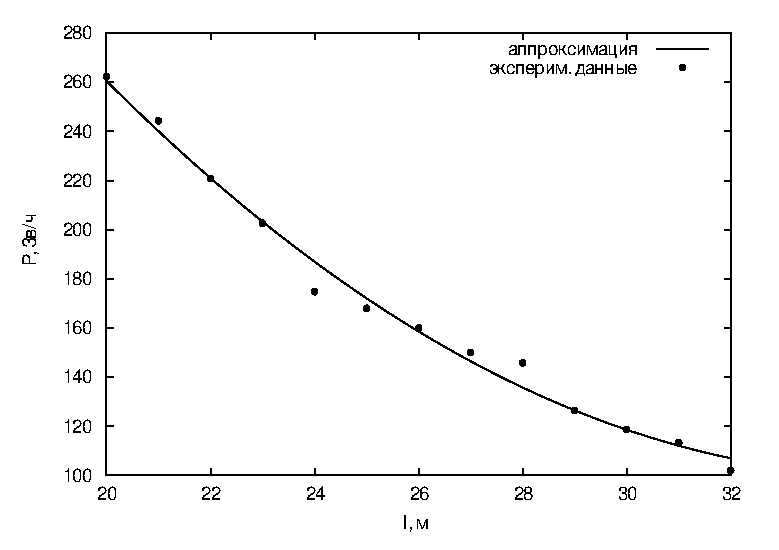
\includegraphics[width=.47\textwidth]{V} \hfill
        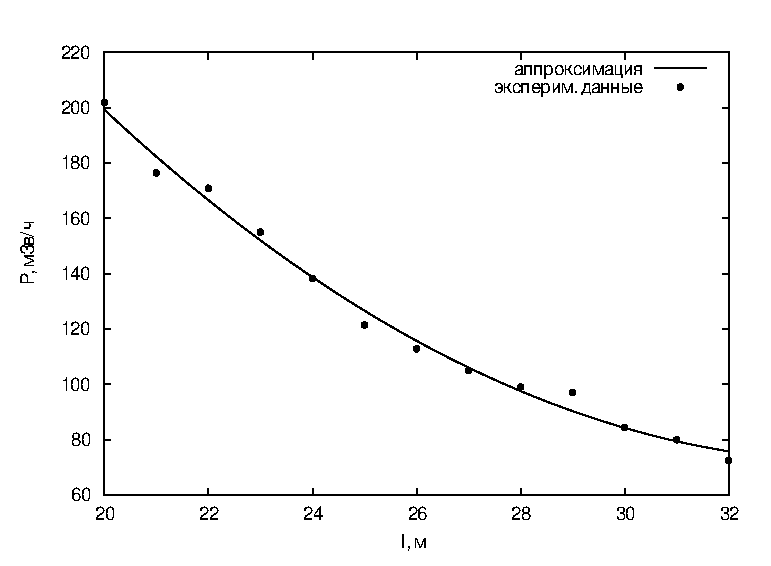
\includegraphics[width=.47\textwidth]{Cs}
        \parbox{.47\textwidth}{\caption{График зависимости \( \midnum{P}(l) \)
        для Ванадия-48}} \hfill
        \parbox{.47\textwidth}{\caption{График зависимости \( \midnum{P}(l) \)
        для Цезия-137}}
    \end{figure}

    \pagebreak % ---------------------------------------------------------------
    
    \subsection{Цинк-65 \( \left(^{65}\mathrm{Zn}\right) \)}
    
    \begin{table}[h!]
        \center
        \begin{tabular}{|C{.065}|*{13}{C{.047}|}} \hline
            \( l \), м & 20 & 21 & 22 & 23 & 24 & 25 & 26 & 27 & 28 & 29 & 30
            & 31 & 32 \\ \hline
            % -------------------------------------------------------
            \multirow{3}{*}{\( P \), Зв/ч} & 6,55 & 6,32 & 5,95 & 5,19 & 4,88
            & 4,87 & 4,07 & 4,00 & 3,60 & 3,37 & 3,36 & 3,13 & 2,83 \\
            \cline{2-14}
            & 6,87 & 5,96 & 5,56 & 4,91 & 4,58 & 4,52 & 4,39 & 3,98 & 3,57
            & 3,33 & 3,13 & 2,98 & 2,65 \\ \cline{2-14}
            & 6,67 & 6,49 & 6,29 & 5,62 & 4,75 & 4,60 & 4,17 & 4,10 & 3,52
            & 3,08 & 3,08 & 3,02 & 2,66 \\ \hline
            Среднее & 6,70 & 6,26 & 5,93 & 5,24 & 4,74 & 4,66 & 4,21 & 4,03
            & 3,56 & 3,26 & 3,19 & 3,04 & 2,71 \\ \hline
            \multirow{3}{*}{\( P \), Р/ч} & 769,85 & 645,41 & 567,41 & 518,64
            & 515,90 & 450,62 & 395,79 & 388,85 & 356,44 & 327,47 & 321,20
            & 318,85 & 304,65 \\ \cline{2-14}
            & 749,22 & 703,69 & 599,52 & 599,50 & 588,36 & 508,43 & 472,54
            & 401,58 & 340,62 & 330,26 & 326,25 & 319,13 & 286,01 \\
            \cline{2-14}
            & 766,37 & 663,50 & 568,53 & 563,01 & 470,19 & 457,32 & 437,46
            & 372,47 & 356,52 & 355,62 & 296,21 & 283,42 & 273,39 \\ \hline
            Среднее & 770,81 & 670,87 & 576,64 & 560,38 & 510,69 & 472,12
            & 435,26 & 387,63 & 351,19 & 337,78 & 314,55 & 307,13 & 288,02 \\
            \hline
        \end{tabular}
    \end{table}
    
    \subsection{Ксенон-133 \( \left(^{133}\mathrm{Xe}\right) \)}
    
    \begin{table}[h!]
        \center
        \begin{tabular}{|C{.065}|*{13}{C{.047}|}} \hline
            \( l \), м & 20 & 21 & 22 & 23 & 24 & 25 & 26 & 27 & 28 & 29 & 30
            & 31 & 32 \\ \hline
            % -------------------------------------------------------
            \multirow{3}{*}{\( P \), Зв/ч} & 56,41 & 45,59 & 45,21 & 37,96
            & 37,01 & 30,66 & 30,54 & 28,80 & 25,23 & 22,99 & 22,79 & 21,14
            & 20,48 \\ \cline{2-14}
            & 55,88 & 43,71 & 42,40 & 38,82 & 36,93 & 31,79 & 29,18 & 27,82
            & 25,87 & 24,66 & 22,75 & 22,20 & 21,24 \\ \cline{2-14}
            & 54,55 & 43,92 & 39,70 & 38,93 & 35,66 & 34,76 & 32,44 & 26,02
            & 25,09 & 22,90 & 21,65 & 20,01 & 18,81 \\ \hline
            Среднее & 55,61 & 44,41 & 42,44 & 38,57 & 36,53 & 32,40 & 30,72
            & 27,55 & 25,73 & 23,52 & 22,40 & 21,12 & 20,18  \\ \hline
            \multirow{3}{*}{\( P \), кР/ч} & 6,02 & 5,34 & 4,99 & 4,06 & 3,91
            & 3,77 & 3,46 & 3,39 & 2,84 & 2,73 & 2,61 & 2,18 & 2,17 \\
            \cline{2-14}
            & 5,40 & 5,38 & 4,93 & 4,04 & 3,75 & 3,73 & 3,59 & 3,41 & 3,10
            & 2,53 & 2,52 & 2,44 & 2,32 \\ \cline{2-14}
            & 6,17 & 5,06 & 4,45 & 4,18 & 3,75 & 3,54 & 3,45 & 3,30 & 3,10
            & 2,85 & 2,69 & 2,53 & 2,24 \\ \hline
            Среднее & 5,86 & 5,26 & 4,79 & 4,09 & 3,80 & 3,68 & 3,50 & 3,37
            & 3,01 & 2,70 & 2,61 & 2,38 & 2,24 \\ \hline
        \end{tabular}
    \end{table}
    
    \begin{figure}[h!]
        \center
        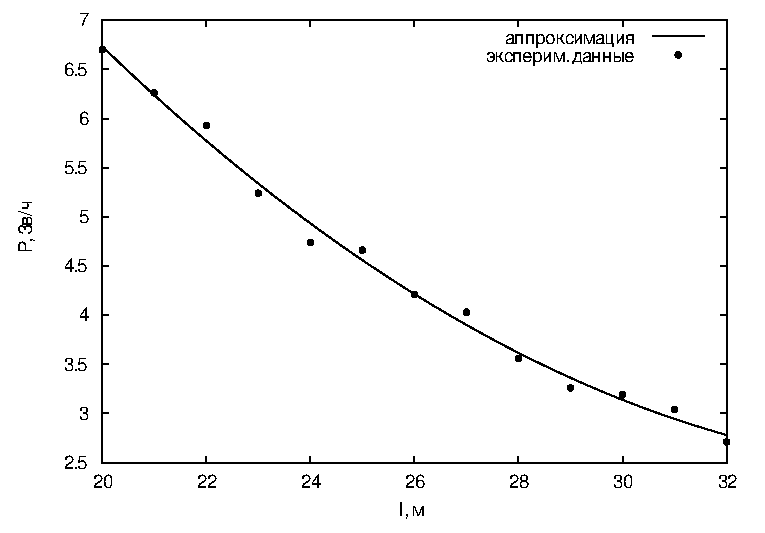
\includegraphics[width=.47\textwidth]{Zn} \hfill
        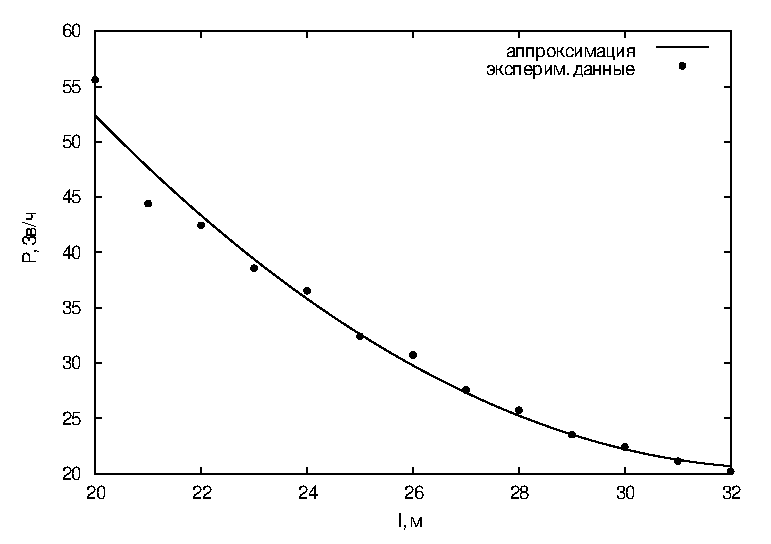
\includegraphics[width=.47\textwidth]{Xe}
        \parbox{.47\textwidth}{\caption{График зависимости \( \midnum{P}(l) \) для Цинка-65}} \hfill
        \parbox{.47\textwidth}{\caption{График зависимости \( \midnum{P}(l) \) для Ксенона-133}}
    \end{figure}

    \emph{Вывод:} провел опыт, моделирующий излучение радиоактивных изотопов, и
    измерил дозу этого излучения при различных расстояниях до источника.
\end{document}
